%!TEX program = xelatex
\documentclass[11pt]{article}
\author {Terry Liu 刘骏杰 l630005038 \\
Section: Dr.Hua-Jun YE}
\title {Regression Assignment Two}
\usepackage{ctex}
\usepackage{amsmath}
\usepackage{amssymb}
\usepackage{color}
\usepackage{amsmath}
\usepackage{graphicx}
\usepackage{float}
\usepackage{listings} %插入代码
\usepackage{xcolor} %代码高亮
\lstset{language=r,
  basicstyle=\ttfamily,
  keywordstyle=\color{blue},
  commentstyle=\color{darkgreen},
  stringstyle=\color{red}}

% change the style of the caption numbering.
\renewcommand{\thetable}{\alph{table}}
\renewcommand{\thefigure}{\Alph{table}}
\renewcommand{\thesubtable}{\Roman{subtable}}
\renewcommand{\thesubfigure}{\arabic{subfigure}}

\begin{document}
\maketitle
\date
  \paragraph{\color{red}{Question One Answer:}}
  For $\sigma = 2$, we can notice that: \\
  \begin{align*}
    p(y) &= Pr(\theta = 1)p(y|\theta = 1) + Pr(\theta = 2)p(y|\theta = 2) \\
    &= 0.5N(y|1,2^2) + 0.5N(y|2,2^2)
  \end{align*}
  The graph can be drawn by R:
  \begin{lstlisting}[language ={R}]
  y <- seq(-7,10,.02)
  density <- 0.5*dnorm(y,1,2) + 0.5*dnorm(y,2,2)
  plot (y, density, ylim=c(0,1.1*max(density)))
  \end{lstlisting}
  The plot is : \\
  \begin{figure}[H] %H为当前位置,!htb为忽略美学标准,htbp为浮动图形
    \centering %图片居中
    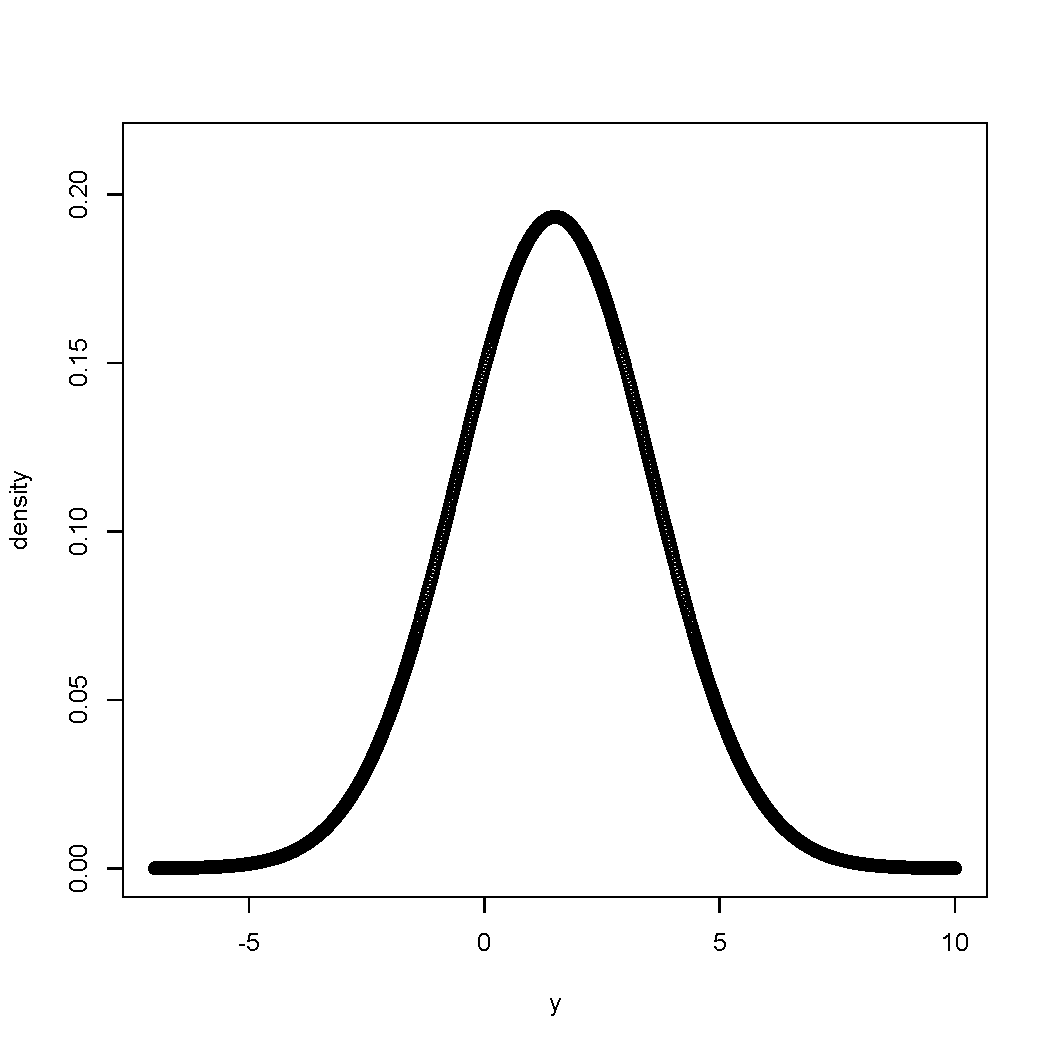
\includegraphics[width=0.3\textwidth]{Rplot} %插入图片,[]中设置图片大小,{}中是图片文件名
    \caption{Marginal probability density of y} %最终文档中希望显示的图片标题
    \label{Fig1} %用于文内引用的标签
  \end{figure}
  \\
  \\
  (b) \\
  \begin{align*}
    Pr(\theta = 1|y = 1) &= \frac{p(\theta=1,\ y = 1)}{p(\theta = 1,\ y = 1) + p(\theta = 2, \ y = 1)} \\
    &= \frac{Pr(\theta = 1)p(y = 1 | \theta = 1)}{Pr(\theta = 1)p(y = 1|\theta = 1) + Pr(\theta = 2)p(y - 1|\theta = 2)} \\
    &= \frac{0.5N(1|1,2^2)}{0.5N(1|1,2^2) + 0.5N(1|2,2^2)} \approx 0.62
  \end{align*}
  \\
  \\
  (c) If $\sigma \rightarrow \infity$, the posterior density for $\theta$ will approaches to the prior density and the probability will be $\frac{1}{2}$; if $\sigma \rightarrow 0$ the $0.5N(1|2,\theata^2) \approx 0$ so the $Pr(\beta = 1| y = 1) \rightarrow 1$.
  \\
  \paragraph{\color{red}{Question Two Answer:}}
  From the question, we can notice that: $Pr(fraternal twins) = \frac{1}{125}$ and $Pr(identical twins) = \frac{1}{300}$. Since the fraternal twins are in different perm cell. the $Pr(both boys) = \frac{1}{4}$\\
  The conditional probability that Elvis was an identical twins is :
  \begin{align*}
    Pr(identical twins | twins brother) &= \frac{Pr(identical twins, \ twins brother)}{Pr(twins brother)} \\
    &= \frac{\frac{1}{2} \times \frac{1}{300}}{\frac{1}{2} \times \frac{1}{300} + \frac{1}{4}\times \frac{1}{125}} \\
    &= \frac{5}{11} \approx 45.5\%
  \end{align*}
  \paragraph{\color{red}{Question Three Answer:}}

  \paragraph{\color{red}{Quesion Four Answer:}}
  (a) The prior predictive distribution for $y$: \\
  \begin{align*}
    Pr(y = k) &= \int^1_0 Pr(y = k|\theta) d\theta \\
    &= \int^1_0 \binom{n}{k} \theta^k(1-\theta)^{n-k}d\theta \\
    &= \binom{n}{k}\frac{\Gamma(k+1)\Gamma(n-k+1)}{\Gamma(n+2)} = \frac{1}{n+1}
  \end{align*}
  \\
  \\
  (b) \ We can notice that the posterior mean is $\frac{\alpha + y}{\alpha + \beta + n}$. We assume that $\lambda \in (0,1)$ and $\frac{\alpha + y}{\alpha + \beta + n} = \lambda \frac{\alpha}{\alpha + \beta} + (1- \lambda)\frac{y}{n}$\\
  \begin{align*}
    \frac{\alpha + y}{\alpha + \beta + n} &= \lambda \frac{\alpha}{\alpha + \beta} + (1- \lambda)\frac{y}{n} \\
    \frac{\alpha + y}{\alpha + \beta + n} - \frac{y}{n} &= \lambda (\frac{\alpha}{\alpha + \beta} - \frac{y}{n}) \\
    \lambda &= \frac{\alpha + \beta}{\alpha + \beta + n}
  \end{align*}
  \\
  \\
  (c) \ When we consider the uniform distribution, we can notice that $\alpha = \beta = 1$, so the prior variance is $\frac{\alpha \beta}{(\alpha + \beta)^2(\alpha + \beta + 1)} = \frac{1}{12}$. In this situation, we can calculate the posterior variance:\\
  \begin{align*}
    \text{Posterior Variance} &= \frac{(1 + y)(1+n-y)}{(2+n)^2(3+n)} \\
    &= (\frac{1+y}{2+n})(\frac{1+n-y}{2+n})(\frac{1}{3+n})
  \end{align*}
  The sum of $\frac{1+y}{2+n}$ and $\frac{1+n-y}{2+n}$ is not greater than $\frac{1}{4}$. And $n \geq 1$, so $\frac{1}{3+n}$ is less than $\frac{1}{4}$. So Posterior vairance $\neq \frac{1}{16}$
  \\
  \\
  (d) \ If $n = 2$,$y = 1$,$\alpha = 1$ and $\beta = 1$ The prior vaiance = $\frac{1}{12}$ and the posterior variance is $0.025$
\end{document}
